\documentclass[12pt, a4paper]{article}

\usepackage{array}
\usepackage[portuguese]{babel}
\usepackage{chngpage}
\usepackage{float}
\usepackage[a4paper, margin=2cm]{geometry}
\usepackage{graphicx}
\usepackage{hyperref}
\usepackage{setspace}
\usepackage{xcolor}

\title{\Huge \textbf{Computação Gráfica \\ \Large Trabalho Prático -- Fase I}}
\date{2 de março 2025}
\author{Grupo \textbf{\color{red} TODO}}

\begin{document}

\begin{center}
    
\includegraphics[width=0.25\textwidth]{res/cover/EE-C.eps}
\end{center}

\chardef\_=`_
\onehalfspacing
\setlength{\parskip}{\baselineskip}
\setlength{\parindent}{0pt}
\def\arraystretch{1.5}

{\let\newpage\relax\maketitle}
\maketitle
\thispagestyle{empty}

\vspace*{\fill}

\begin{adjustwidth}{-2cm}{-2cm} % These values only need to be large enough to center the table
    \begin{center}
        \begin{tabular}{>{\centering}p{0.25\textwidth}
                        >{\centering}p{0.25\textwidth}
                        >{\centering}p{0.25\textwidth}
                        >{\centering\arraybackslash}p{0.25\textwidth}}
            
\includegraphics[width=3.5cm]{res/cover/A104437.png} &
            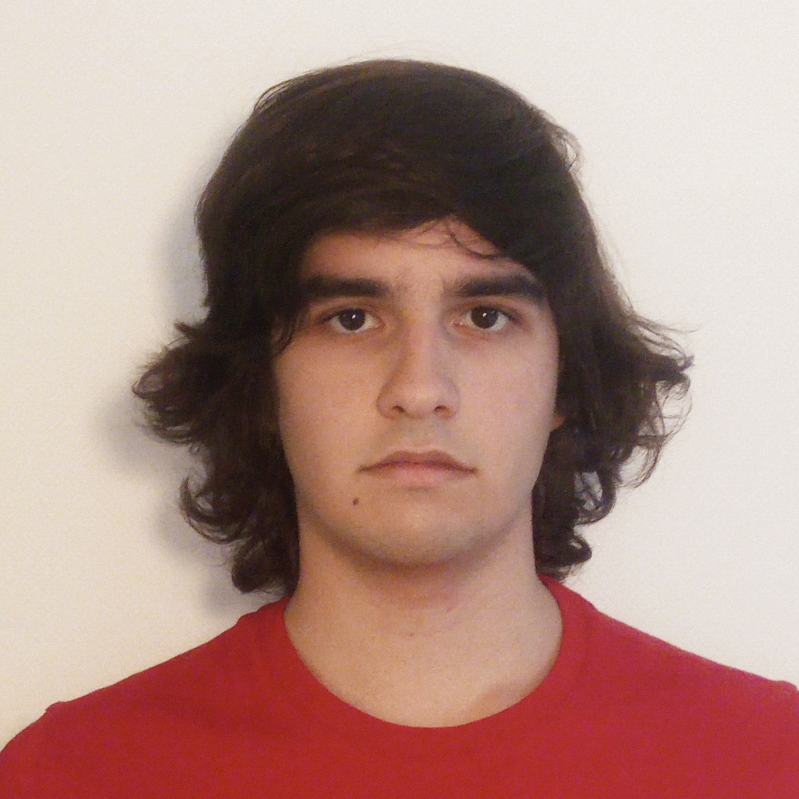
\includegraphics[width=3.5cm]{res/cover/A104348.png} &
            
\includegraphics[width=3.5cm]{res/cover/A90817.png} &
            
\includegraphics[width=3.5cm]{res/cover/A104179.png} \\

            Ana Oliveira & Humberto Gomes & Mariana Cristino & Sara Lopes \\
            A104437      & A104348        & A90817           & A104179
        \end{tabular}
    \end{center}
\end{adjustwidth}

\pagebreak

\begin{abstract}
    \textbf{\color{red} TODO - resumo}
\end{abstract}

\section{\emph{Generator}}

\subsection{Descrição e uso}

\textbf{\color{red} TODO - descrição e uso do programa}

\subsection{Formato do \emph{output}}

\textbf{\color{red} TODO - formato do \emph{output}}

\subsection{Plano}

O processo de criação do modelo 3D de um plano é dividido em duas fases: a geração do conjunto de
pontos que o constitui, e o seu agrupamento em faces triangulares. Esta divisão tem origem na
estrutura de um ficheiro \texttt{.3d}, que separa os vértices de um modelo das suas faces.

O primeiro passo para a geração da nuvem de pontos de um plano é o cálculo do comprimento de uma
divisão, $d = \frac{L}{N}$, onde $L$ simboliza o comprimento do plano e $N$ o número de divisões.
Depois, determinam-se os dois vetores que definem a direção do plano. Estes poderiam ser os vetores
diretores dos eixos $x$ e $z$, mas é mais simples que estes tenham o comprimento de uma divisão do
plano.

$$
\vec{\imath} = (s, 0, 0)
\hspace{1cm}
\vec{\jmath} = (0, 0, s)
$$

Depois, encontra-se o ponto do plano com os menores valores das coordenadas $x$ e $z$. Como se
deseja que o plano esteja centrado na origem, as coordenadas $x$ e $z$ do ponto desejado serão o
simétrico da metade do comprimento do plano:

$$
P_0 = \left ( - \frac{S}{2}, 0, - \frac{S}{2} \right )
$$

Depois, qualquer ponto $P$ do plano pode ser definido como a adição a $P_0$ de uma combinação linear
de $\vec{\imath}$ e $\vec{\jmath}$, limitando a números inteiros os coeficientes multiplicativos dos
vetores:

$$
P = P_0 + \alpha \, \vec{\imath} + \beta \, \vec{\jmath}
\hspace{1cm}
\alpha, \beta \in \left \lbrace 0, 1, \ldots, N \right \rbrace
$$

Na prática, o plano é gerado iterando pelos valores inteiros possíveis de $\alpha$ e de $\beta$,
incrementando primeiro $\beta$, e só depois de $\alpha$, o que dá origem a uma nuvem de pontos como
a que pode ser observada na figura abaixo:

\begin{figure}[H]
    \centering
    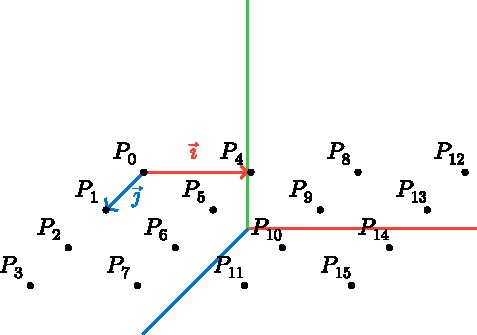
\includegraphics[width=0.4\textwidth]{res/figures/PlanePoints.pdf}
    \caption{Nuvem de pontos resultante da geração de um plano de três divisões.}
\end{figure}

Depois, os vértices gerados podem ser agrupados nos triângulos que formam o plano. Para tal,
começa-se com o primeiro vértice do plano, $P_0$. Considera-se também o vértice seguinte, $P_1$, e
os dois vértices com os valores de $z$ de $P_0$ e $P_1$, mas com o seguinte valor de $x$ possível
(na "linha"{} seguinte). Um exemplo de um conjunto destes quatro vértices pode ser visto na figura
abaixo. Com estes vértices, gera-se um quadrado, ou seja, dois triângulos. Este processo repete-se
para todos os vértices onde é aplicável, ou seja, todos com exceção dos pontos com os maiores
valores de $x$ ou de $z$ possíveis.

\begin{figure}[H]
    \centering
    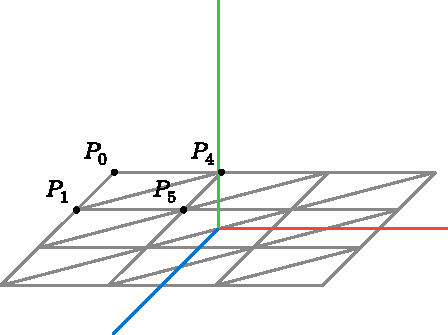
\includegraphics[width=0.4\textwidth]{res/figures/PlaneTriangles.pdf}
    \caption{
        Triângulos de um plano gerado, e pontos utilizados na primeira iteração do ciclo de geração
        de triângulos.
    }
\end{figure}

Uma otimização feita pela \emph{engine} é \emph{face culling}, ou seja, desenhar apenas as faces
voltadas para a câmara. No caso do plano, deseja-se que os seus triângulos estejam voltados para
cima, pelo que os seus vértices devem estar ordenados na ordem contrária à dos ponteiros do
relógio. Para os quatro pontos apresentados acima, os triângulos gerados são os seguintes:

$$
T_1 = (P_1, P_4, P_0)
\hspace{1cm}
T_2 = (P_1, P_5, P_4)
$$

\section{\emph{Engine}}

\textbf{\color{red} TODO - \emph{engine}}

\section{Resultados obtidos}

\textbf{\color{red} TODO - resultados}

\section{Conclusão e Trabalho Futuro}

\textbf{\color{red} TODO - conclusão}

\begingroup
\section{Bibliografia}
\renewcommand{\section}[2]{}

\begin{thebibliography}{9}
    \bibitem{exemplo}
        \href{https://youtu.be/dQw4w9WgXcQ}{Um item de exemplo na bibliografia}
\end{thebibliography}
\endgroup

\end{document}
